\documentclass[]{tesis-pregrado}

\keywords{AI; CNN; Deep Learning, Machine Learning}

\begin{document}
    \baselineskip 23pt
    
    % ----------- PORTADA Y CUBIERTAS --------------------------------
    \thispagestyle{empty}
    \titulo{Formato de Tesis, en Latex, para el Departamento de Física, USACH}
\autor{Student Studentsson}  % nombre del alumno
%\email{}
%\telefono{}
%\run{}
%\annoingreso{}
\fecha{}{}{Mayo}{2021}
\profesorguia{Professor Professorson}  % nombre del profesor
\profesorcoguia{}
\diploma{Diploma Diplomasson}  % título profesional
\ciudad{Santiago -}
\pais{Chile}
\makecubierta
  % Portada 1
    \thispagestyle{empty}

\noindent Si su trabajo de titulación forma parte de un proyecto financiado con fondos públicos,
indique aquí:

\vspace*{0.5cm}

\noindent Tipo Proyecto --- Número --- Título del Proyecto.




  % portada 2 si hay fondos involucrados
    \thispagestyle{empty}
\begin{center}

\vspace*{1.5cm}
\LARGE{\bf{Formato de Tesis, en Latex, para el Departamento de Física, USACH}} \par

\vspace*{2.5cm}

{\large\bf Student Studentsson}\\[1.0cm]

\vspace*{1.0cm}
\normalsize
Este trabajo de graduación fue elaborado bajo la supervisión del profesor
patrocinante Professor Professorson y ha sido aprobado por los miembros de la
comisión calificadora.
\end{center}

\vspace*{2.5cm}


\begin{flushright}
\begin{minipage}{8.8cm}
Professor Professorson 2 \hrulefill \\ \\
Professor Professorson 3 \hrulefill
\end{minipage}
\end{flushright}

\vspace*{4cm}

\begin{flushleft}
\begin{minipage}{7.5cm}
  \centering
  \hrulefill\\
  Professor Professorson \\
  % Director del Departamento de Física\\
\end{minipage}
\end{flushleft}


  % portada 3 después de la revisión
    \makecopyright % si acaso será publicado en biblioteca
    \begin{center}
		{\Large\bf DEDICATORIA}
\end{center}

\vfill

geschrieben werden
 

    \begin{center}
		{\Large\bf AGRADECIMIENTOS}
\end{center}

\vfill

geschrieben werden
 

    
    % ----------- RESUMEN Y TABLAS DE CONTENIDO ---------------------
    \frontmatter
    \pagestyle{scrplain}  % scrplain or scrheadings
    
    \resumenCastellano{

\vspace*{0.25cm}

En este trabajo de tesis se han presentado 3 problemas de procesamiento de imágenes utilizando técnicas de aprendizaje profundo para resolverlos. Gracias al poder computacional actual y la evolución en los algoritmos de inteligencia artificial, el campo del procesamiento de imágenes ha sido un gran beneficiado.

\vspace*{0.5cm}

Se ha creado un clasificador de imágenes de radiografías de tórax para identificar Covid-19, Pneumonia y pacientes sanos, la particularidad de esta implementación es que puede ser facilmente modificable para implementarla en cualquier otro tipo de problema de clasificación de imágenes. La implementación está escrita completamente en Python y la red puede ser entrenada tanto en un compilador como en un \emph{jupyter notebook}.

\vfill

\KeywordsES{Aprendizaje Automático, CNN, Rayos X, Detector Facial, YOLO, Detector de mascarillas}

}

\newpage

\resumenIngles{
 
\vspace*{0.25cm}

In this thesis, 3 image processing problems have been presented using deep learning techniques to solve them. Thanks to the current computational power and the evolution of artificial intelligence algorithms, the field of image processing has been a great beneficiary.

\vspace*{0.5cm}

An X-ray chest image classifier has been created to identify Covid-19, Pneumonia and healthy patients, the strong point of this implementation is that it can be easily modified to implement it for any other type of image classification problem. The implementation is written entirely in Python and the network can be trained in both a compiler or in a \emph{jupyter notebook}.

\vfill

\KeywordsEN{Machine Learning, CNN, X-ray, Face Detector, YOLO, Mask Detector}

}


    \tableofcontents        %% Indice general
    \listoftables           %% Indice de tablas
    \listoffigures          %% Indice de figuras
    
    % ----------- CAPITULOS DE LA TESIS --------------------------------
    \mainmatter
    \pagenumbering{arabic}
    
    \setcitestyle{square}  % para las referencias con un número en parentesis de cuadro si se usa IEEEtran, % si se usa IEEEtranN, la referencia es escrita con autor y año
    \chapter{Introducci\'on}
\label{cap:intro}

\section{Antecedentes y motivaci\'on}
\label{intro:motivacion}

geschrieben werden

\section{Objetivos y alcance}
\label{intro:objetivos}


\subsection{Objetivo general}


\subsection{Objetivos espec\'ificos}


\subsection{Alcances}


\section{Metodolog\'ia y herramientas utilizadas}
\label{intro:metodologia}

\subsection{Metodolog\'ia}

\subsection{Herramientas de desarrollo}

\section{Casos de Estudio}
\label{intro:casos_estudio}

\subsection{Dataset: Covid-19}

\subsection{Reconocimiento facial}

\subsection{Detector de Objetos: YOLO}


    \chapter{Marco Te\'orico}
\label{cap:preliminares}

\section{Redes Neuronales Artificiales}
\label{intro:redes_neuronales}

Con $n$ entradas en el nodo desde $x_1$ hasta $x_n$ y $\varphi$ la funci\'on de activaci\'on. La salida del nodo n\'umero $j$ es:

\vspace*{0.5cm}

\begin{equation}
y_j = \varphi (\displaystyle\sum_{j=i}^{n} w_{ji} x_i + b_j)
\label{eq:output_network}
\end{equation}

\vspace*{0.5cm}  % espacio entre párrafos 

\begin{figure}[ht]
  \centering
  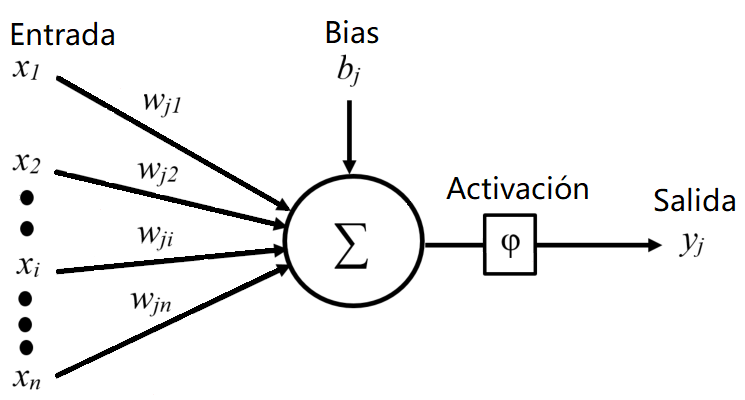
\includegraphics[scale=0.40]{images/neuron_unit_sp.png}
  \caption[Nodo Artificial unitario]{Nodo artificial unitario que imita la estructura cerebral. Su funci\'on es aprender y es un elemento b\'asico de aprendizaje.}
  \label{fig:rna_neuron}
\end{figure}

\clearpage
\section{Funciones de Activaci\'on}
\label{intro:activations}

\subsection{Sigmoide}

Tambi\'en se conoce como funci\'on de activaci\'on log\'istica. Toma un n\'umero de valor real y lo acota en un rango entre 0 y 1. Tambi\'en se usa en la capa de salida donde el objetivo final es predecir una probabilidad. Convierte grandes números negativos en 0 y grandes números positivos en 1. Matem\'aticamente se representa como:

\begin{equation}
\sigma(x) = \frac{1}{1+\mathrm{e}^{-x}}
\label{eq:sigmoide}
\end{equation}

\noindent y su derivada:

\begin{equation}
\frac{\partial}{\partial x} \sigma(x) = \sigma(x)(1-\sigma(x))
\label{eq:sigmoide_derivada}
\end{equation}

\vspace*{0.5cm}

\subsection{LeakyReLU}
\label{leakyrelu_title}

\begin{equation}
\frac{\partial}{\partial x} z(x) = 
\begin{cases}
1   & x > 0 \\
0.1 & x < 0
\end{cases} \label{eq:leaky_derivate}
\end{equation}


\section{M\'etodos de Optimizaci\'on}

\subsection{Descenso del Gradiente Estoc\'astico}

\begin{equation}
W_{t+1} = W_t - \alpha \nabla f(W_t)
\label{eq:sgd}
\end{equation}

\vspace*{0.3cm}

donde $\alpha$ es la tasa de aprendizaje y $\nabla f(W_t)$ es el gradiente (o derivada) de la funci\'on de p\'erdida con respecto de $W$.


\section{Propagaci\'on hacia atr\'as (\emph{Backpropagation})}

Es una t\'ecnica utilizada para realizar eficientemente el descenso del gradiente en una red neuronal \citep{10.5555/65669.104451}.


\section{M\'aquinas de Soporte Vectorial (\emph{support-vector machine})}
\label{intro:svm}

Las M\'aquinas de Soporte Vectorial (\emph{SVM}) son de los algoritmos m\'as populares en Machine Learning. Estos suelen utilizarse en problemas de clasificaci\'on, regresi\'on, e incluso detecci\'on de valores at\'ipicos (\emph{outliers}). El m\'etodo de soporte vectorial fue presentado por Boser, Guyon y Vapnik \citep{boser1992} en la Conferencia ACM de Teoría del Aprendizaje Computacional (COLT92).

\vspace*{0.5cm}

La idea de construir un hiperplano separador \'optimo en un contexto no-param\'etrico, desarrollado por Vapnik y Chervonenkis \citep{Vapnik:1964} y por Cover \citep{4038449}.


\section{Redes Neuronales Convolucionales (\emph{CNN})}
\label{intro:cnns}


\subsection{Capas Convolucionales}


\section{Arquitecturas Comunes}

\subsection{YOLO: You Only Look Once}
\label{teo:yolo}

YOLO fue presentado en el 2016 como un nuevo enfoque para la detecci\'on de objetos. En vez de re-utilizar clasificadores para realizar la detecci\'on, este enmarca la detecci\'on de objectos como un problema de regresi\'on de cajas delimitadores (\emph{bounding box}) espacialmente separadas con una probabilidad asociada. Solo una red neuronal predice cajas delimitadores y probabilidades de las clases directamente desde la imagen completa en una sola evaluaci\'on. De esta manera, esta arquitectura se deshace de complejos diagramas de flujo (\emph{pipelines}) y la hace extremadamente r\'apida \citep{redmon2016look}.

\vspace*{0.5cm}

\begin{table}[h!]
\centering
\begin{tabular}{lccccc}
Columna    & Top-1         & Top-5         & Bn Ops & BFLOP/s       & FPS          \\
\hline
Darknet-19 & 74.1          & 91.8          & 7.29   & 1246          & \textbf{171} \\
Resnet-101 & 77.1          & 93.7          & 19.7   & 1039          & 53           \\
Resnet-152 & \textbf{77.6} & \textbf{93.8} & 29.4   & 1090          & 37           \\
Darknet-53 & 77.2          & \textbf{93.8} & 18.7   & \textbf{1457} & 78          
\end{tabular}
\caption[Comparaci\'on de Columnas Vertebrales]{Comparaci\'on de Darknet-53 con otras columnas vertebrales (\emph{backbones}) de otras arquitecturas.}
\label{table:backbones}
\end{table}

\vspace*{0.5cm}

\begin{table}[ht!]
\centering
\begin{tabular}{l c c c c} 
 & \textbf{Tipo} & \textbf{Filtros} & \textbf{Tamaño}    & \textbf{Salida}    \\
 & Convolutional & 32      & 3 x 3     & 256 x 256 \\
 & Convolutional & 64      & 3 x 3 / 2 & 128 x 128 \\
 & \done Convolutional & \done 32      & \done 1 x 1     & \done          \\
1 x & \done Convolutional & \done 64      & \done 3 x 3     & \done          \\
 & \done Residual      & \done        & \done          & \done 128 x 128 \\
 & Convolutional & 128     & 3 x 3 / 2 & 64 x 64   \\
 & \done Convolutional & \done 64      & \done 1 x 1     & \done          \\
2 x & \done Convolutional & \done 128     & \done 3 x 3     & \done          \\
    & \done Residual      & \done        & \done           & \done 64 x 64   \\
    & Convolutional & 256     & 3 x 3 / 2 & 32 x 32   \\
    & \done Convolutional & \done 128     & \done 1 x 1     & \done          \\
8 x & \done Convolutional & \done 256     & \done 3 x 3     & \done          \\
    & \done Residual      & \done        & \done           & \done 32 x 32   \\
    & Convolutional & 512     & 3 x 3 / 2 & 16 x 16   \\
    & \done Convolutional & \done 256     & \done 1 x 1     & \done          \\
8 x  & \done Convolutional & \done 512     & \done 3 x 3     & \done          \\
     & \done Residual      & \done         & \done          & \done 16 x 16   \\
     & Convolutional & 1024    & 3 x 3 / 2 & 8 x 8     \\
     & \done Convolutional & \done 512     & \done 1 x 1     & \done          \\
4 x  & \done Convolutional & \done 1024    & \done 3 x 3     & \done          \\
     & \done Residual      & \done        & \done           & \done 8 x 8     \\
     & Avgpool       &         & Global    &           \\
     & Connected     &         & 1000      &           \\
     & Softmax       &         &           &
\end{tabular}
\caption{Arquitectura Darknet-53}
\label{table:darknet53}
\end{table}

    \chapter{Implementaci\'on y Resultados}
\label{cap:implementacion}

%%%%%%%%%%%%%% CASO 1
\section{Dataset: Covid-19}
\label{intro:covid}

\subsection{Implementaci\'on}

\begin{lstlisting}[language=python]
total_train = sum(len(files) for _, _, files in os.walk(traindir))
pbar = tqdm(total=total_train, desc='Loading training images')
for d in os.listdir(traindir):
    categories.append(d)
    train_imgs = os.listdir(os.path.join(traindir, d))
    valid_imgs = os.listdir(os.path.join(validdir, d))
    test_imgs = os.listdir(os.path.join(testdir, d))
    n_train.append(len(train_imgs))
    n_valid.append(len(valid_imgs))
    n_test.append(len(test_imgs))

    for i in train_imgs:
        img_categories.append(d)
        img = cv2.imread(os.path.join(traindir, d, i))
        img_array = np.array(img)
        pbar.update(1)
        hs.append(img_array.shape[0])
        ws.append(img_array.shape[1])
pbar.close()

cat_df = pd.DataFrame({'category': categories,
                       'n_train': n_train,
                       'n_valid': n_valid,
                       'n_test': n_test}).\
                        sort_values('category')

cat_df.sort_values('n_train', ascending=False, inplace=True)
\end{lstlisting}

\vspace*{0.5cm}

%%%%%%%%%%%%%%%%%% CASO 2
\clearpage
\section{Reconocimiento Facial} % 
\label{intro:face_detector}

\subsection{Implementaci\'on}

\begin{center}
  \begin{tikzpicture}[node distance=2cm]
    \node (node0) [startstop] {Conjunto de im\'agenes};
    \node (node1) [process, right of=node0, xshift=4cm] {Detecci\'on Facial};
    \node (node2) [process, below of=node1] {Alineaci\'on Facial};
    \node (node3) [process, below of=node2] {Extraer Incrustaciones};
    \node (node4) [fit, below of=node3] {Fitear un SVM con las incrustaciones};
    \node (node5) [startstop, below of=node4] {Reconocimiento facial en im\'agenes y v\'ideos};
    
    \draw [arrow] (node4) --node[anchor=east] {\small{guardar modelo}} (node5);
    \draw [arrow] (node3) --node[anchor=east] {\small{128-d OpenFace}} (node4);
    \draw [arrow] (node2) --node[anchor=east] {\small{68 hitos con DLIB}} (node3);
    \draw [arrow] (node1) --node[anchor=east] {\small{recortar caras}} (node2);
    \draw [arrow] (node0) --node[anchor=south, text width=3.5cm, align=center] {\small{caffemodel}} (node1);
  \end{tikzpicture}
 \vspace*{0.5cm}
\captionof{figure}[Diagrama de flujo detecci\'on facial]{Diagrama de Flujo en la implementaci\'on para el reconocimiento y clasificaci\'on facial}
\label{fig:flowface}
\end{center}

\vspace*{0.5cm}

%%%%%%%%%%%% CASO 3
\clearpage
\section{YOLO: Detector de Mascarillas}  % yolo
\label{imple:yolov5}

\subsection{Implementación}

\subsection{Resultados}
\label{imple:yoloResults}


\begin{figure}[htb]
    \centering % <-- added
\begin{subfigure}{0.45\textwidth}
  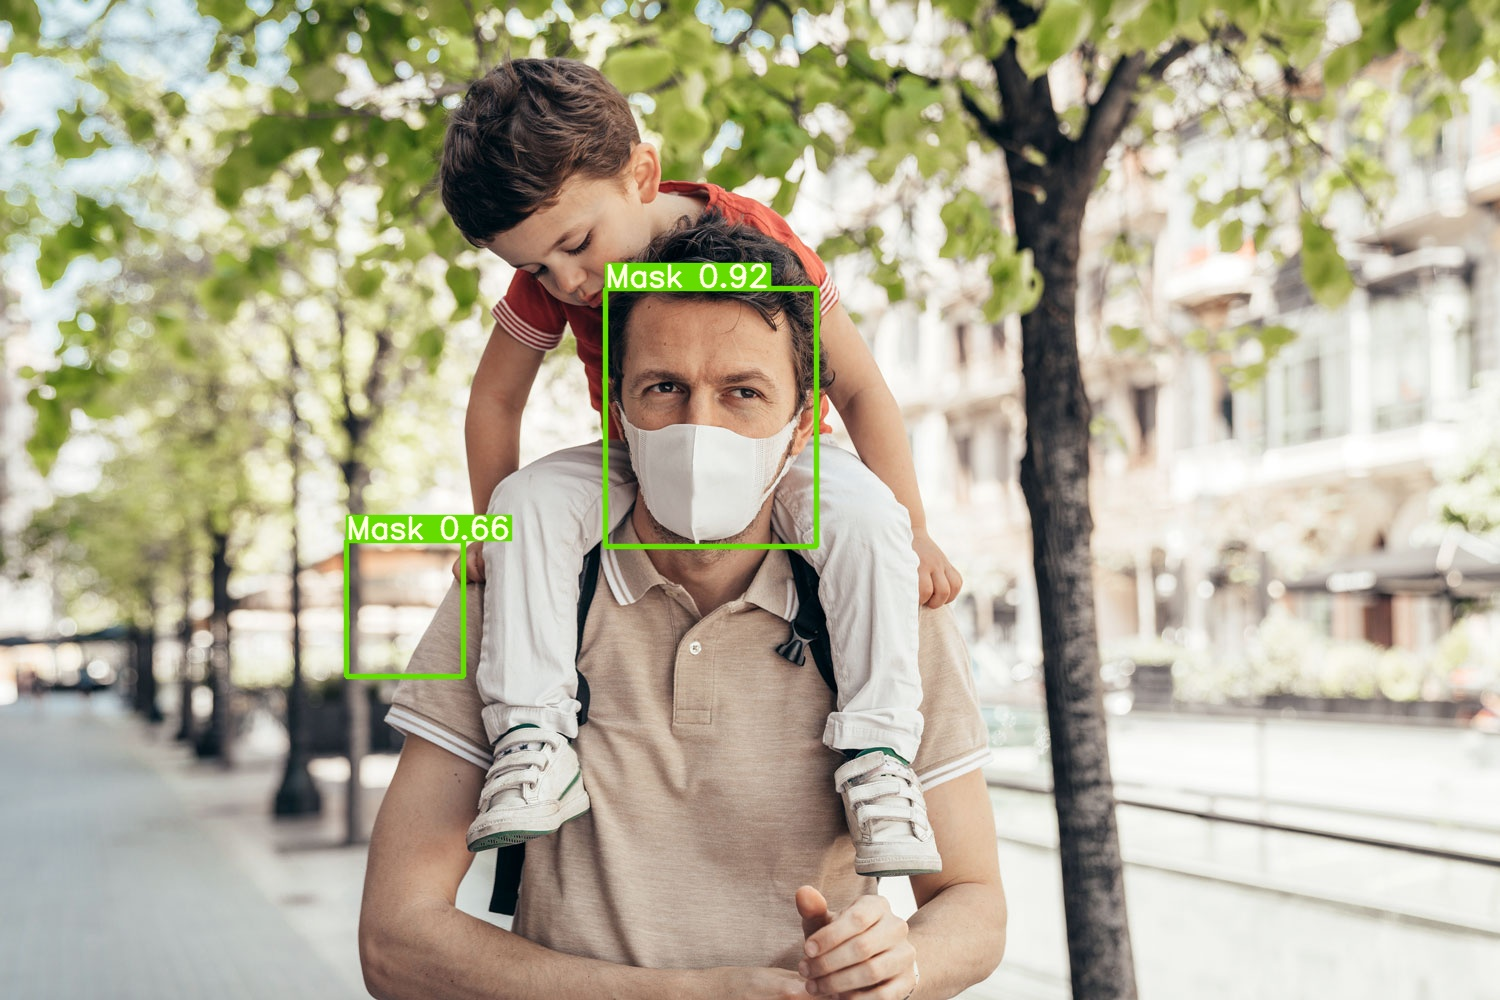
\includegraphics[width=\linewidth]{images/covid_test5.jpg}
  \caption{Hay una sobredetección de un rostro con mascarilla y una baja detección de un rostro sin mascarilla.}
  \label{fig:1}
\end{subfigure}\hfil % <-- added
\begin{subfigure}{0.45\textwidth}
  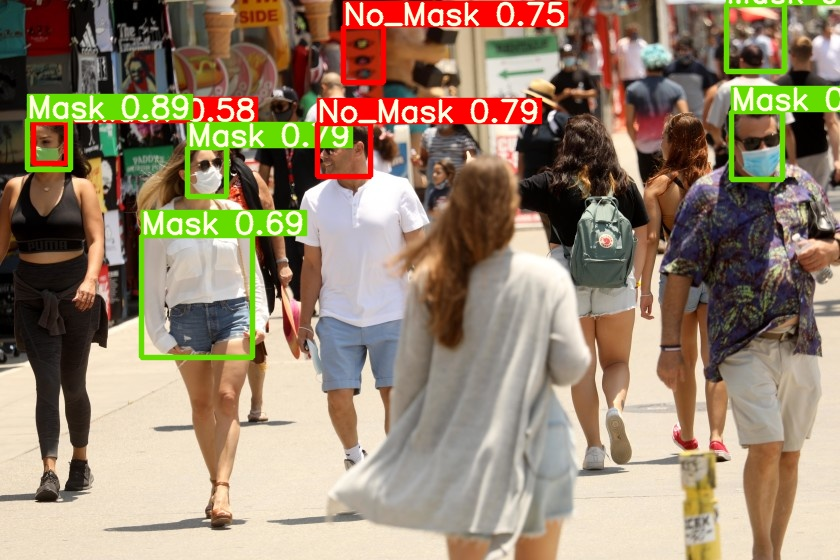
\includegraphics[width=\linewidth]{images/covid_test2.jpg}
  \caption{Hay una sobredetección, No-Mask, sobre una detección correcta, esto se podría corregir con un umbral mayor de Non-maximum Suppression.}
  \label{fig:2}
\end{subfigure}\hfil % <-- added

\medskip
\begin{subfigure}{0.45\textwidth}
  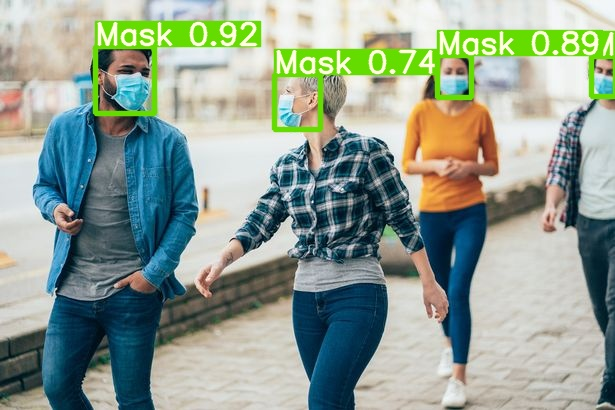
\includegraphics[width=\linewidth]{images/covid_test6.jpg}
  \caption{Todas las personas usando mascarillas se han detectado correctamente.}
  \label{fig:4}
\end{subfigure}\hfil % <-- added
\begin{subfigure}{0.45\textwidth}
  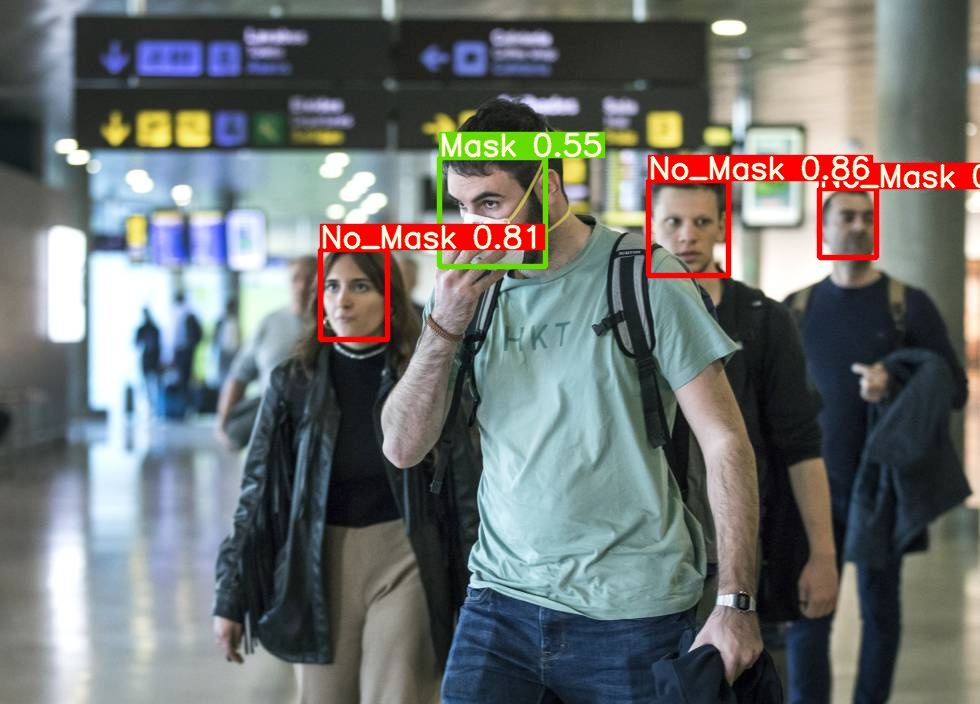
\includegraphics[width=\linewidth]{images/covid_test8.jpg}
  \caption{Se he detectado correctamente las personas con y sin mascarillas.}
  \label{fig:5}
\end{subfigure}\hfil % <-- added
\caption[Imágenes de pruebas]{Imágenes reservadas para pruebas. Aunque las métricas del modelo son bastante favorables, en producción, el modelo podría tener un error mucho más alto. La única manera de corregirlo es aumentar la cantidad de datos de entrenamiento recopilando más imágenes y anotaciones.}
\label{fig:yolotests}
\end{figure}
    \chapter*{Conclusiones}
\addcontentsline{toc}{chapter}{Conclusiones} 

geschrieben werden
    
    % ----------- REFERENCIAS BIBLIOGRAFICAS --------------------------------
    % \backmatter %Elimina la numeración
    \bibliographystyle{IEEEtran}  % chapters/apa-good, or IEEEtranN
    \bibliography{chapters/referencias}  % referencias.bib

    % ----------- ANEXOS ---------------------------------
    \appendix
    \addappheadtotoc %agregar Apéndice al índice. Si no tiene apéndices COMENTAR o BORRAR
    % \noappendicestocpagenum %quitar número de páginas a los apéndices
    \chapter{Apéndice}
\label{cap:manual}

geschrieben werden




 % Manuales de Usuario
\end{document}
